%===========================================================
\chapter{Genome and Inheritance}
%===========================================================

\section{The six-gene body genome}
Every animal carries an immutable \code{Genome}: an ordered vector of six bounded
quantitative traits,
\[
\mathbf{g}=(\text{size},\ \text{speed},\ \text{perception},\ \text{metabolism},\ \text{reproduction\_threshold},\ \text{fertility}),
\qquad g_i\in[L_i,H_i].
\]
Each value must be finite and inside its configured bounds; a genome built from a
mapping must contain exactly these six keys.

\begin{table}[htbp]
\centering
\caption{Body genes and their effects}
\begin{tabularx}{\textwidth}{lL}
\toprule
Gene & Effect in the model \\
\midrule
size & Raises basal and movement cost; strengthens contests and defence. \\
speed & Faster travel and access; raises movement cost and travel utility cost. \\
perception & Radius for sensing food, mates, threats; does not guarantee capture. \\
metabolism & Divides basal cost: higher metabolism means \emph{better} basal efficiency in this code base. \\
reproduction\_threshold & Energy an animal must hold to be eligible to mate. \\
fertility & Shortens mating cooldown: $\max(1,\mathrm{round}(c(1-0.5f)))$. \\
\bottomrule
\end{tabularx}
\end{table}

\subsection{Founders}
Each founder gene is drawn independently and uniformly, $g_i\sim U(L_i,H_i)$.

\subsection{Crossover}
Two operators are configurable. \emph{Arithmetic} crossover draws an independent
$\alpha_i\sim U(0,1)$ per gene and sets
\[
c_i=\alpha_i a_i+(1-\alpha_i)b_i,
\]
so offspring lie between their parents. \emph{Uniform} crossover takes each gene
from one parent with probability $1/2$.

\subsection{Mutation}
Independently per gene, a Bernoulli trial with probability $p_m$ gates a Gaussian
perturbation scaled to the gene's span, then the value is clamped:
\[
g'_i=\mathrm{clamp}_{[L_i,H_i]}\big(c_i+\varepsilon_i\big),\qquad
\varepsilon_i\sim\mathcal{N}\big(0,\ \sigma(H_i-L_i)\big)\ \text{with prob. } p_m.
\]
The showcase uses $p_m=0.1$ and $\sigma=0.075$, so a mutated gene typically moves
by 7.5\% of its range.

\section{Temperament}
Aggression, resilience and sociability are inherited separately from the body
genome, each in $[0,1]$. Offspring values combine the parental values with seeded
Gaussian variation and are clipped to $[0,1]$. Aggression raises contest risk and
strength; resilience reduces exposure injury and strengthens defence; sociability
raises mating and care drives and influences tradition founding.

\section{The opt-in diploid architecture}
\code{config/diploid-biome.json} enables an explicit chromosome model. It is an
unreleased research preview; the default showcase does not use it.

Each animal carries two phased binary haplotypes $h^{(1)},h^{(2)}\in\{0,1\}^L$
with $2\le L\le64$ loci on one linked chromosome. Expression proceeds in three
steps. First, a dominance-adjusted dosage per locus,
\[
\delta_\ell=\frac{h^{(1)}_\ell+h^{(2)}_\ell}{2}+d_\ell\,\frac{|h^{(1)}_\ell-h^{(2)}_\ell|}{2},
\qquad d_\ell\in[-1,1].
\]
Second, each trait's effect row $\mathbf{e}_j$ is normalised to unit absolute mass
and applied around the midpoint,
\[
n_j=\mathrm{clip}\Big(0.5+\sum_\ell \frac{e_{j\ell}}{\sum_k|e_{jk}|}\,(\delta_\ell-0.5)\Big).
\]
Third, the trait is mapped into its bounds: $g_j=L_j+n_j(H_j-L_j)$.

Meiosis starts on a random homologue and switches homologue in interval $\ell$
with probability $r_\ell\in[0,0.5]$, producing one recombinant gamete per parent.
Founders draw each allele as 1 with the configured founder frequency. Figure
\ref{fig:diploid} shows the preview's allele frequencies, heterozygosity, linkage
association and individual dosages.

\begin{figure}[htbp]
\centering
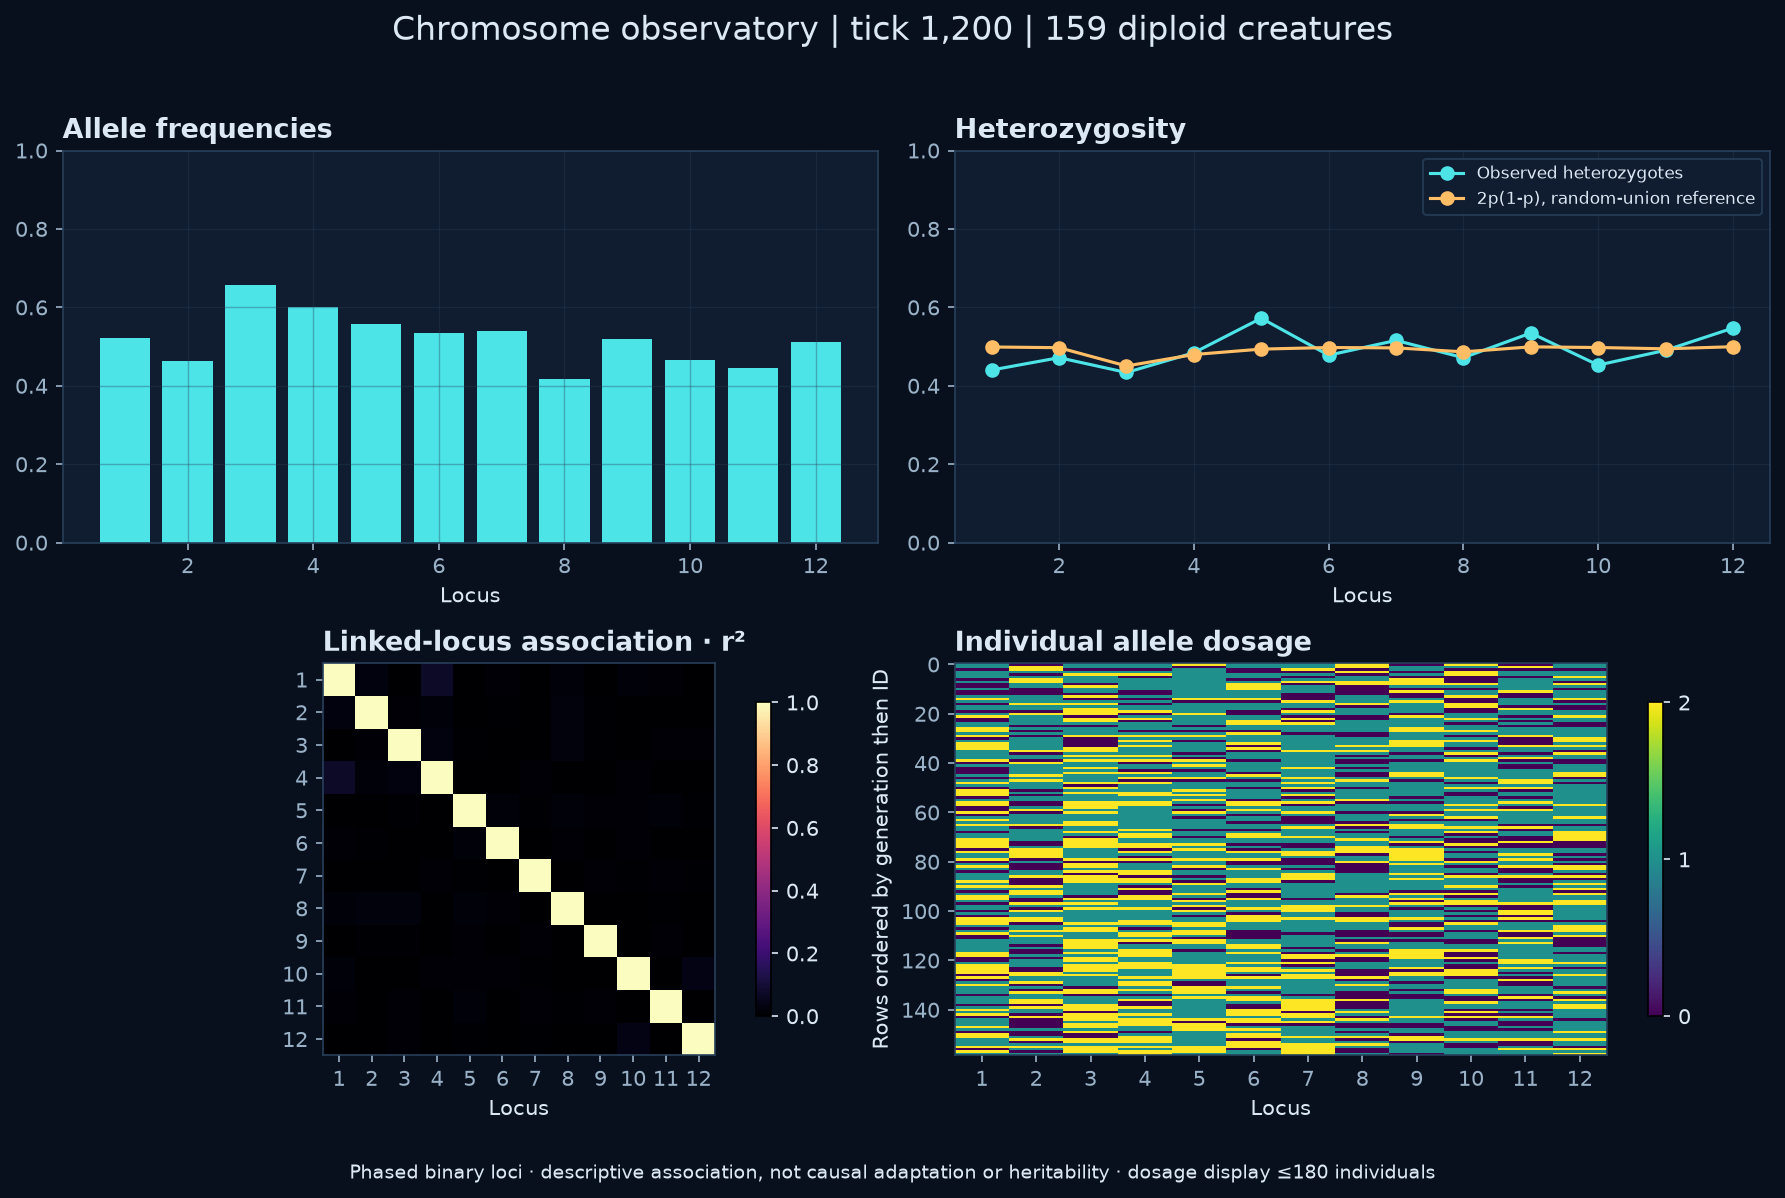
\includegraphics[width=0.92\textwidth]{chromosomes.png}
\caption{Diploid preview (seed 2026, tick 1{,}200): allele frequencies,
heterozygosity against the $2p(1-p)$ reference, linked-locus $r^2$ and individual
dosages. One development run; not long-horizon validation.}
\label{fig:diploid}
\end{figure}

\section{Heritable thermal optimum}
When climate forcing is enabled, each animal also carries a thermal optimum
$\theta$ in $^{\circ}$C, clamped to $[-20,60]$. Founders draw
$\theta\sim\mathcal{N}(\mu_f,\sigma_f)$ where $\mu_f$ defaults to the local annual
mean plus the starting anomaly and $\sigma_f=1\,^{\circ}$C. Offspring follow the
infinitesimal model:
\[
\theta_{\text{child}}=\frac{\theta_1+\theta_2}{2}+\mathcal{N}(0,\sigma_s)+\mathcal{N}(0,\sigma_\mu),
\qquad \sigma_s=0.4,\ \sigma_\mu=0.1.
\]
With \code{inheritance = "none"} the offspring optimum is instead drawn afresh from
the founder distribution: the control arm has the same spread but zero heritability.

%===========================================================
\chapter{Behaviour: Drives, Utilities and Arbitration}
%===========================================================

\section{Perception}
Each decision receives a tick-local perception: food patches, eligible mates,
threats and dependent offspring within the animal's perception radius, plus global
hazard and terrain pressures and the animal's own home-range displacement. The
perception is a contract: behaviour never reads the world directly.

\section{The six drives}
Drives are normalised pressures in $[0,1]$, stored and displayed in a fixed order.
With $E$ the energy, $E_{\max}$ the maximum and $I$ the injury:
\begin{align*}
\text{deficit}&=\mathrm{clip}(1-E/E_{\max})\\
\text{survival}&=\mathrm{clip}\big(0.65(1-E/E_{\max})+0.35I\big)\\
\text{hunger}&=\max(\text{stored\_hunger},\ \text{deficit})\\
\text{foraging}&=\mathrm{clip}\big(\text{hunger}\,(0.5+0.5\,\text{best\_food\_reward})\big)\quad\text{if food is sensed, else }0\\
\text{danger}&=\max(\text{local\_hazard},\ \text{best\_threat\_pressure})
\end{align*}
Food reward is
$\mathrm{clip}\big(\text{food\_energy}/\max(1,0.15E_{\max})\big)\cdot\mathrm{clip}(1-\text{distance}/\text{perception})$.
Threat pressure combines proximity, the threat's aggression, relative size and the
receiver's injury, each bounded to $[0,1]$.

\textbf{Mating} is zero unless the animal and at least one perceived mate are
eligible, survival is below 0.55 and injury below 0.65; otherwise
\[
\text{mating}=\mathrm{clip}\big((0.5+0.5E/E_{\max})\cdot\text{proximity}\cdot(0.7+0.3\,\text{sociability})\big).
\]
\textbf{Offspring care} is the maximum over nearby dependents $j$ of
\begin{multline*}
\mathrm{clip}\big(0.35(1-\text{age}_j/\text{dependent\_age})+0.45\,\mathrm{clip}(1-E_j/E_{\max})\\
+0.20\max(I_j,\text{danger})\big)\cdot(0.6+0.4\,\text{sociability}).
\end{multline*}
\textbf{Territory}, with $d$ the distance from the home centre and $r$ the home radius:
\[
\text{territory}=\mathrm{clip}(0.35+0.65\,d/r)\,(1-0.75\,\text{hunger})\,(1-0.5\,\text{danger}).
\]

\begin{figure}[htbp]
\centering
\begin{minipage}{0.49\textwidth}\centering
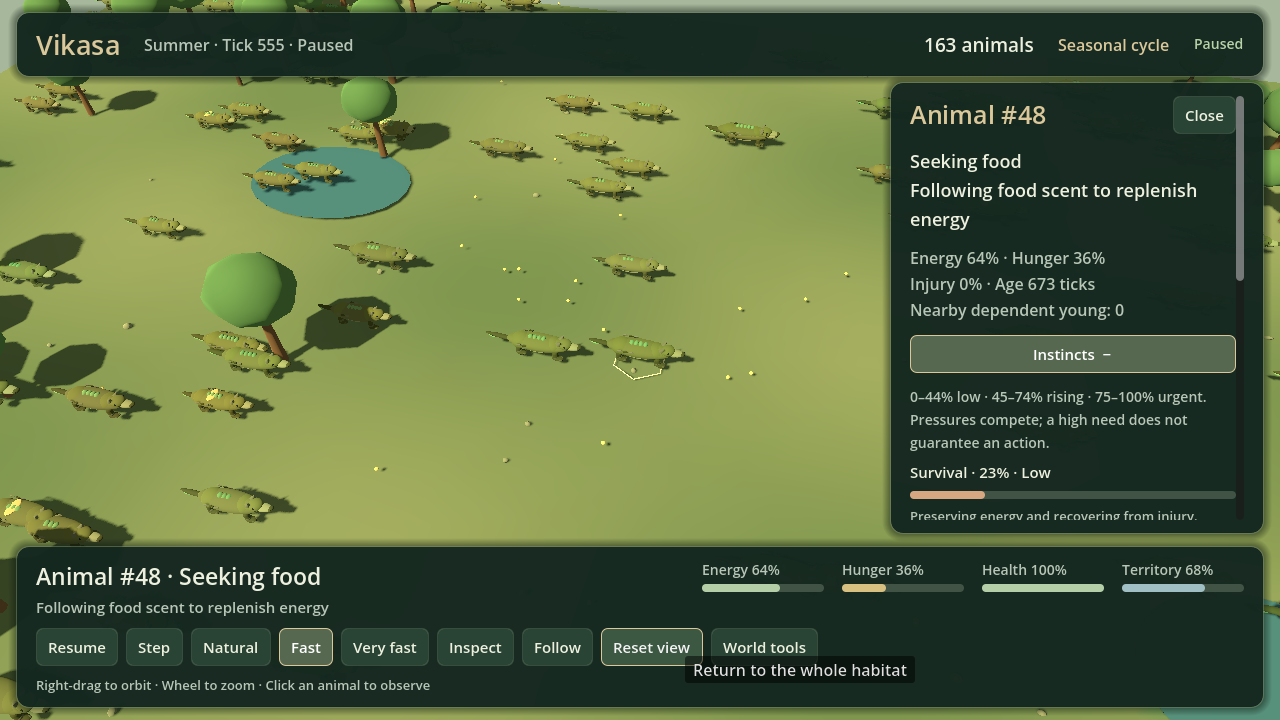
\includegraphics[width=\linewidth]{wildlife-instincts.png}\\[-2pt]
{\small (a) Instincts panel}
\end{minipage}\hfill
\begin{minipage}{0.49\textwidth}\centering
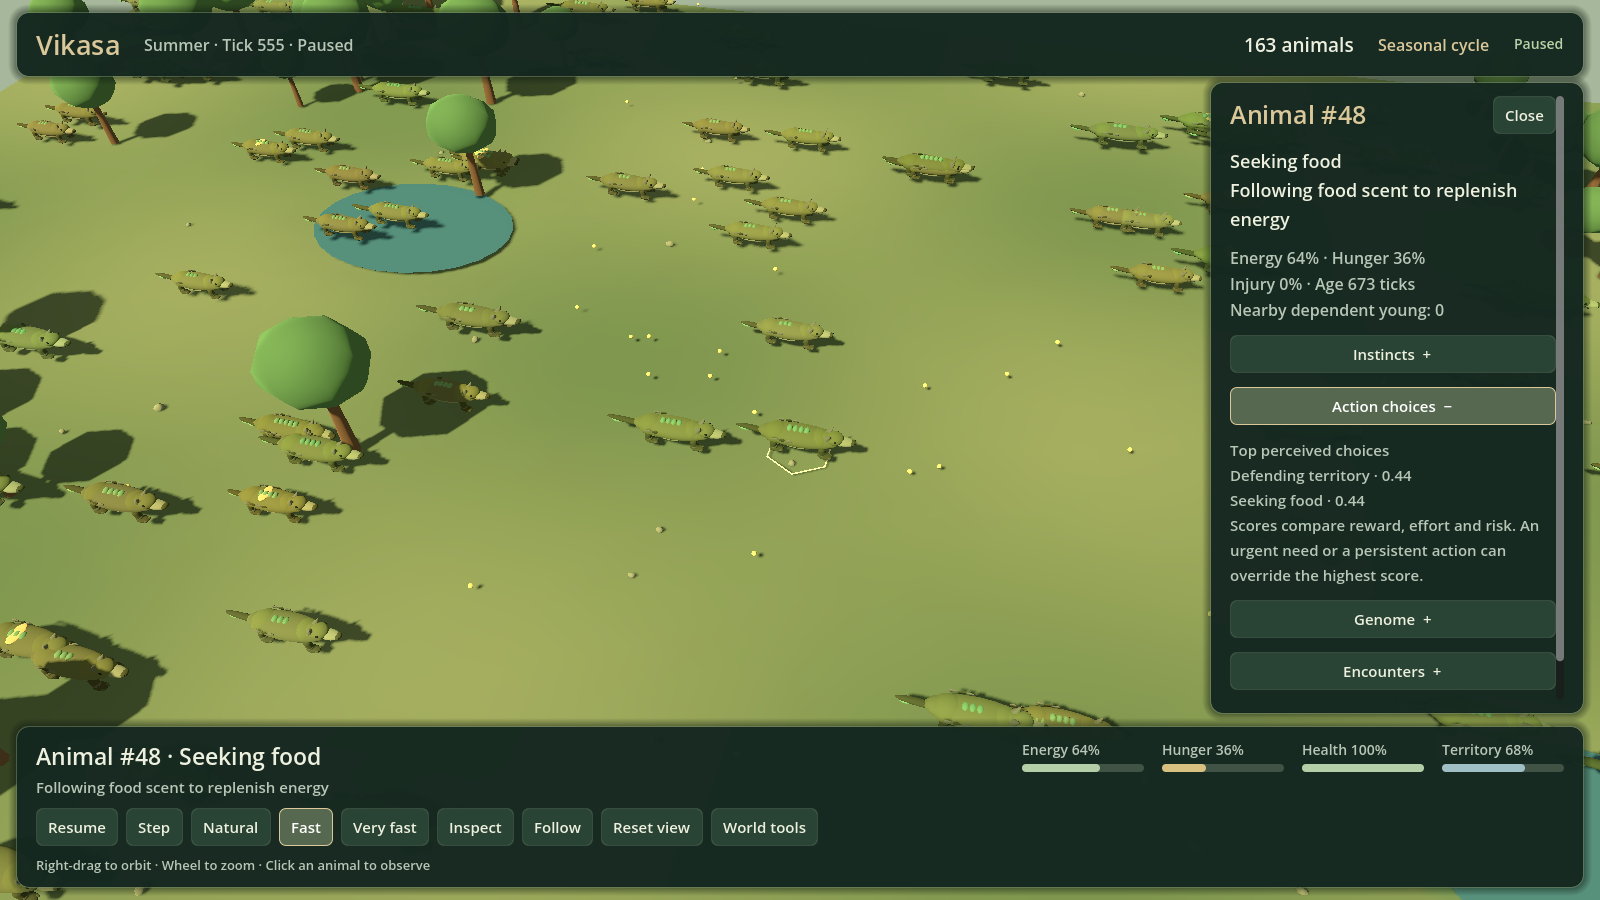
\includegraphics[width=\linewidth]{wildlife-action-choices.png}\\[-2pt]
{\small (b) Action choices panel}
\end{minipage}
\caption{The inspector exposes the six drives and the leading action utilities.}
\end{figure}

\section{Action utilities}
Eight actions compete. For action $a$ with affinity vector $\mathbf{A}_a$ over the
six drives $\mathbf{D}$:
\[
U_a=\mathrm{clip}\Big(\textstyle\sum_k A_{a,k}D_k+R_a-T_a-X_a-K_a\Big)
\]
where $R_a$ is an action-specific reward (local food value, relief from survival
pressure, dependent need, danger or territory context) and the costs are
\begin{align*}
T_a&=0.12\,\mathrm{clip}(\text{distance}/\text{perception})\,\frac{\text{speed}/4}{\text{metabolism}}+0.08\,\text{terrain\_cost}\quad(\text{not for rest})\\
X_a&=\begin{cases}0.05\,\text{danger}&\text{rest}\\0&\text{flee}\\0.25\,\text{danger}&\text{otherwise}\end{cases}\qquad
K_a=\begin{cases}0.15\,\text{danger}&\text{seek mate}\\0.30\,\text{danger}/\text{relative strength}&\text{challenge}\\0&\text{otherwise.}\end{cases}
\end{align*}

\begin{table}[htbp]
\centering
\caption{Action affinities over (survival, foraging, mating, care, danger, territory)}
\begin{tabular}{lcccccc}
\toprule
Action & Surv. & Forage & Mate & Care & Danger & Terr. \\
\midrule
explore & 0.10 & 0.15 & 0 & 0 & 0 & 0 \\
forage & 0.35 & 0.65 & 0 & 0 & 0 & 0 \\
rest & 0.55 & 0 & 0 & 0 & 0 & 0 \\
seek mate & 0 & 0 & 0.65 & 0 & 0 & 0 \\
care & 0 & 0 & 0 & 0.75 & 0 & 0 \\
flee & 0.15 & 0 & 0 & 0 & 0.85 & 0 \\
patrol & 0 & 0 & 0 & 0 & 0 & 0.65 \\
challenge & 0 & 0 & 0 & 0 & 0 & 0.45 \\
\bottomrule
\end{tabular}
\end{table}

\section{Arbitration}
\begin{enumerate}[leftmargin=*]
\item Actions without a valid opportunity (no food, no mate, no dependent, no
rival) are \emph{excluded}, not given a fabricated competing score.
\item Danger at or above the preemption threshold (0.75) forces \emph{flee}.
\item Survival pressure at or above 0.65 forces \emph{forage} when food is sensed,
otherwise \emph{explore}. Injury at or above 0.65 forces \emph{rest}.
\item Otherwise the current action is retained if its utility is within the
hysteresis margin (0.08) of the best candidate, which prevents jitter.
\item Remaining near-ties within the softmax temperature $\tau$ are resolved with
seeded probabilities $P(a)=\exp((U_a-U_{\max})/\tau)/\sum_j\exp((U_j-U_{\max})/\tau)$.
\end{enumerate}
High need therefore does not guarantee the matching action: opportunity, travel,
danger, conflict, preemption and persistence all matter. Each decision records the
action, its target, the start tick, the full utility breakdown and a
human-readable reason (at most 240 characters). The base reasons are: explore
``Searching nearby for better habitat'', forage ``Following food scent to replenish
energy'', rest ``Resting to conserve energy and recover'', seek mate ``Approaching an
eligible mate'', care ``Staying near hungry or vulnerable young'', flee ``Moving away
from danger'', patrol ``Returning toward the home range'' and challenge ``Defending
the home range under local competition''.

\section{Home range, patrol, care and migration}
Each animal has a home-range centre and a radius (sampled deterministically per
creature). \emph{Patrol} chooses a persistent waypoint near the range edge.
\emph{Care} lets a parent feed living offspring younger than the dependent age and
within the care radius, transferring a limited amount of energy while protecting
the parent's own reserve. \emph{Migration} is a small local-resource response: if
an animal remains outside its range while foraging, and the perceived outside food
reward exceeds the inside reward by the migration margin (0.15) for 24 consecutive
qualifying ticks, its centre shifts 0.5\% toward its position.

%===========================================================
\chapter{Energy, Survival and Mortality}
%===========================================================

\section{Energy budget}
Basal expenditure per tick is
\[
C_b=c_b\,\frac{1+\text{size}/8}{\text{metabolism}}\;
\mu_{\text{event}}\,\mu_{\text{season}}\,\mu_{\text{injury}}\,\mu_{\text{health}}\,(1+1.5\,\varsigma),
\]
where the last factor applies only with climate forcing. Movement expenditure is
\[
C_m=c_m\cdot\text{distance}\cdot(0.5+\text{size}/8)\,(0.5+\text{speed}/4)\cdot\mu_{\text{weather}}.
\]
Energy is clamped at $E_{\max}$ after food gain and costs. Food is consumed once
and supplies the patch's remaining energy; competing animals resolve access by
squared distance, then stable ID.

\section{Starvation}
Hunger is $\mathrm{clip}(1-E/E_{\max})$. At non-positive energy a starvation
counter increases by one per tick; when energy is positive it decreases by one, to
a floor of zero. Death occurs at 12 accumulated starvation ticks. Starvation is
therefore delayed and reversible, not a single-tick deletion.

\section{Exposure injury}
Under health pressure $H$ (from weather events, Chapter~\ref{ch:env}) injury rises
by
\[
\Delta I=0.018\,H\,(1-0.75\,\text{resilience})\,(1+0.6\,\text{hunger}),\qquad I'=\min(1,I+\Delta I).
\]
Lethal injury is $I\ge0.98$. With active health pressure it is attributed to
environmental exposure, otherwise to fight injuries; with mixed causes the
attribution is approximate. Calm-weather recovery is unchanged.

\section{Thermal stress}
With climate forcing (Chapter~\ref{ch:climate}) thermal stress $\varsigma$ is
computed in the energy step before the basal cost. It multiplies the basal cost by
$1+1.5\varsigma$, adds injury $0.02(\varsigma-0.3)/0.7$ per tick when
$\varsigma>0.3$, and blocks reproduction while $\varsigma>0.7$.

\section{Age-dependent mortality}
Optional Gompertz mortality uses a piecewise-constant per-tick hazard
\[
\mu(a)=\mu_0\exp\big(b\max(0,a-a_0)\big),\qquad
P(\text{death in tick}\mid\text{alive})=1-e^{-\mu(a)},\qquad
S(A)=\prod_{a<A}e^{-\mu(a)}.
\]
The engine computes in log space and caps the hazard at 50, where per-tick
survival is already below $2\times10^{-22}$. A seeded uniform draw decides
mortality after the injury and starvation checks. With $\mu_0=0$ stochastic
senescence is disabled and no extra draws are consumed. The hard
\code{maximum\_age} ceiling (12{,}000 ticks in the showcase) remains a safety
bound, not an expected lifespan.

\begin{figure}[htbp]
\centering
\begin{tikzpicture}
\draw[->] (0,0) -- (11,0) node[right]{\small age (ticks)};
\draw[->] (0,0) -- (0,4.2) node[above]{\small $S(a)$};
\foreach \x/\l in {0/0,2/1000,4/2000,6/3000,8/4000,10/5000} \draw (\x,0.08)--(\x,-0.08) node[below]{\scriptsize \l};
\foreach \y/\l in {0/0,2/0.5,4/1.0} \draw (0.08,\y)--(-0.08,\y) node[left]{\scriptsize \l};
\draw[thick,vk,domain=0:3.6,samples=40] plot (\x,{4*exp(-0.00002*\x*500)});
\draw[thick,vk,domain=3.6:10,samples=200] plot (\x,{4*exp(-0.036 - 0.01*(exp(0.002*(\x*500-1800))-1))});
\draw[dashed,gray] (3.6,0) -- (3.6,4) node[above,font=\scriptsize]{$a_0=1800$};
\end{tikzpicture}
\caption{Gompertz survivorship $S(a)$ for the showcase parameters
($\mu_0=2\times10^{-5}$, $b=0.002$, $a_0=1800$), ignoring starvation, injury and
the age ceiling.}
\end{figure}

\section{Why the lifecycle changed}
The earlier showcase, preserved as \code{config/extinction-control.json}, used a
fixed 1{,}100-tick lifespan. For seed 2026 it reached zero animals by tick 3{,}000
with only 25 births, 69 old-age deaths and 20 starvation deaths; at tick 1{,}500
only 11 animals remained. Same-aged founders were removed by the hard limit before
they could be replaced, and encounter density, neonatal reserves and resource
production further constrained replacement. The current showcase changes the world
size, founder and newborn reserves, mating radius, resource production and
mortality model together; it adds no immigration, rescue, restart or death
suppression.

%===========================================================
\chapter{Reproduction, Conflict, Satisfaction and Culture}
%===========================================================

\section{Reproduction}
Both partners must be mutually selected, within the mate radius, old enough,
above their reproduction-threshold energy, off cooldown, and below the population
cap; with climate forcing, both must also have thermal stress at most 0.7. Each
parent contributes half the configured offspring energy. The child inherits the
body genome (crossover and mutation), temperament, and the thermal optimum, and its
parentage and birth tick enter the lineage store, where they remain after the
parents die. Effective cooldown is $\max(1,\mathrm{round}(c\,(1-0.5f)))$ for base
cooldown $c$ and fertility $f$.

\section{Contests}
Fights are deliberately rare. A contest is only possible at close range under
hunger pressure of at least 0.48 or during an active challenge, and fleeing
prevents it. Encounter risk starts at
\[
p=0.004\,(0.25+\text{pressure})\,(0.3+\overline{\text{aggression}}),
\]
is multiplied by 1.5 for a challenge and by $1+0.75\,s_{\text{fights}}$ for an
active challenger (with $s_{\text{fights}}$ the fight component of satisfaction),
and is capped at 0.09; ordinary maximum-pressure challenge risk remains below 0.03.
Strength combines size, aggression and current energy; defence combines size and
resilience. Both participants pay energy; the loser gains injury and pays more.
Lethal risk is bounded by 0.42 and rises with low post-contest energy and injury.
The winner gains \emph{alpha} status and increments its fight wins. There is no
permanent rank hierarchy.

\section{Satisfaction}
Satisfaction is an inspectable summary, not fitness:
\begin{align*}
s_E&=\mathrm{clip}(E/E_{\max}), & s_O&=1-e^{-\text{offspring}/3},\\
s_F&=1-e^{-\text{food}/\max(1,\,8\cdot\text{energy\_value})}, & s_W&=1-e^{-\text{wins}/2},\\
S&=0.34s_E+0.18s_O+0.22s_F+0.26s_W.
\end{align*}
Only the fight component feeds back, modestly raising repeat-challenge utility and
the low encounter risk.

\section{Culture: cue-based traditions}
The \code{CultureLedger} implements a small rule-based cultural transmission
mechanism. After each tick it collects shared \emph{signals}: a season turn every
96 ticks, active drought, heat or storm events, and any victory. A signal counts as
a new occurrence only if more than 8 ticks have passed since its last occurrence,
and every living animal accumulates exposure to it.

When a signal has occurred at least 3 times and no tradition for it exists, and at
least 5 animals are alive, a seeded draw with probability 0.012 per tick may found
a tradition. At least 5 animals must have been exposed to the signal 3 or more
times; the founder is the exposed animal with the highest
$\text{sociability}+0.15\cdot\text{fights\_won}$ (ties broken by lower ID). Affiliation then
spreads through low-probability contact, gatherings record rituals, and followers
are pruned as they die.

\begin{table}[htbp]
\centering
\caption{Tradition vocabulary}
\begin{tabularx}{\textwidth}{llL}
\toprule
Signal & Tradition & Ritual \\
\midrule
season-turn & The Turning & mark the changing season \\
drought & Keepers of the Deep & remember the returning water \\
heat & The Shade Circle & gather beneath shelter at noon \\
storm & Voices Before Rain & call together before the storm \\
victory & The First Hunt & honor a victorious elder \\
\bottomrule
\end{tabularx}
\end{table}

\note{This demonstrates rule-based transmission only. It does not model language,
agency, theology, symbolic reasoning or human religion, and a tradition may not
emerge in a particular run.}

%===========================================================
\chapter{Environment and Weather}
\label{ch:env}
%===========================================================

\section{Seasons}
Without climate forcing a season lasts 96 ticks and a year 384 ticks. With
forcing the season index follows the climate year. Each season sets a normalised
temperature (without forcing), rainfall, a food multiplier and a metabolic multiplier.

\begin{table}[htbp]
\centering
\caption{Seasonal signals}
\begin{tabular}{lcccc}
\toprule
Season & Temperature index & Rainfall & Food multiplier & Metabolic multiplier \\
\midrule
spring & 0.58 & 0.76 & 1.12 & 0.96 \\
summer & 0.82 & 0.38 & 0.96 & 1.04 \\
autumn & 0.55 & 0.62 & 0.84 & 0.98 \\
winter & 0.30 & 0.52 & 0.72 & 1.14 \\
\bottomrule
\end{tabular}
\end{table}

\section{Scheduled events}
Events have a kind, start tick, positive duration, positive finite intensity and an
optional label. Contributions from simultaneous events compose: food and
metabolic multipliers multiply, health pressure and resource decay add.

\begin{longtable}{p{2cm}p{12.4cm}}
\caption{Event effects for intensity $I$}\\
\toprule
Event & Effects \\
\midrule
\endfirsthead
\toprule
Event & Effects \\
\midrule
\endhead
drought & Food $\times I$ (intensity is food growth retained; lower is harsher). With severity $s=\max(0,1-I)$: decay $+0.035s$, metabolism $\times(1+0.8s)$, health $+0.15s$, rainfall $\times\min(1,I)$. \\
abundance & Food $\times I$. \\
heat & Metabolism $\times I$; health $+0.45\max(0,I-1)$; decay $+0.012\max(0,I-1)$; temperature index $+0.15I$ (capped at 1). \\
cold & Metabolism $\times I$; health $+0.25\max(0,I-1)$; temperature index $-0.15I$ (floored at 0). \\
storm & Movement cost $\times I$; health $+0.35I$; decay $+0.012I$; rainfall $+0.2I$ (capped at 1). \\
flood & Food $\times\max(0.1,1/I)$; health $+0.45I$; decay $+0.025I$. \\
wildfire & Food $\times\max(0.05,1-0.75I)$; health $+0.8I$; decay $+0.055I$. Whole-biome exposure, not a moving fire front. \\
disease & Health $+0.4I$. Pressure, not explicit contagion. \\
redistribute & Relocates food (world-tool support). \\
\bottomrule
\end{longtable}

Existing food decays each tick as $e'=e\,(1-\min(0.4,\text{decay}))$, and a patch
below 1 energy unit is removed. In the 3D client, World tools apply these events
with a chosen intensity and duration (default 160 ticks); \emph{Restart biome}
resets the population with the same seed.

\begin{figure}[htbp]
\centering
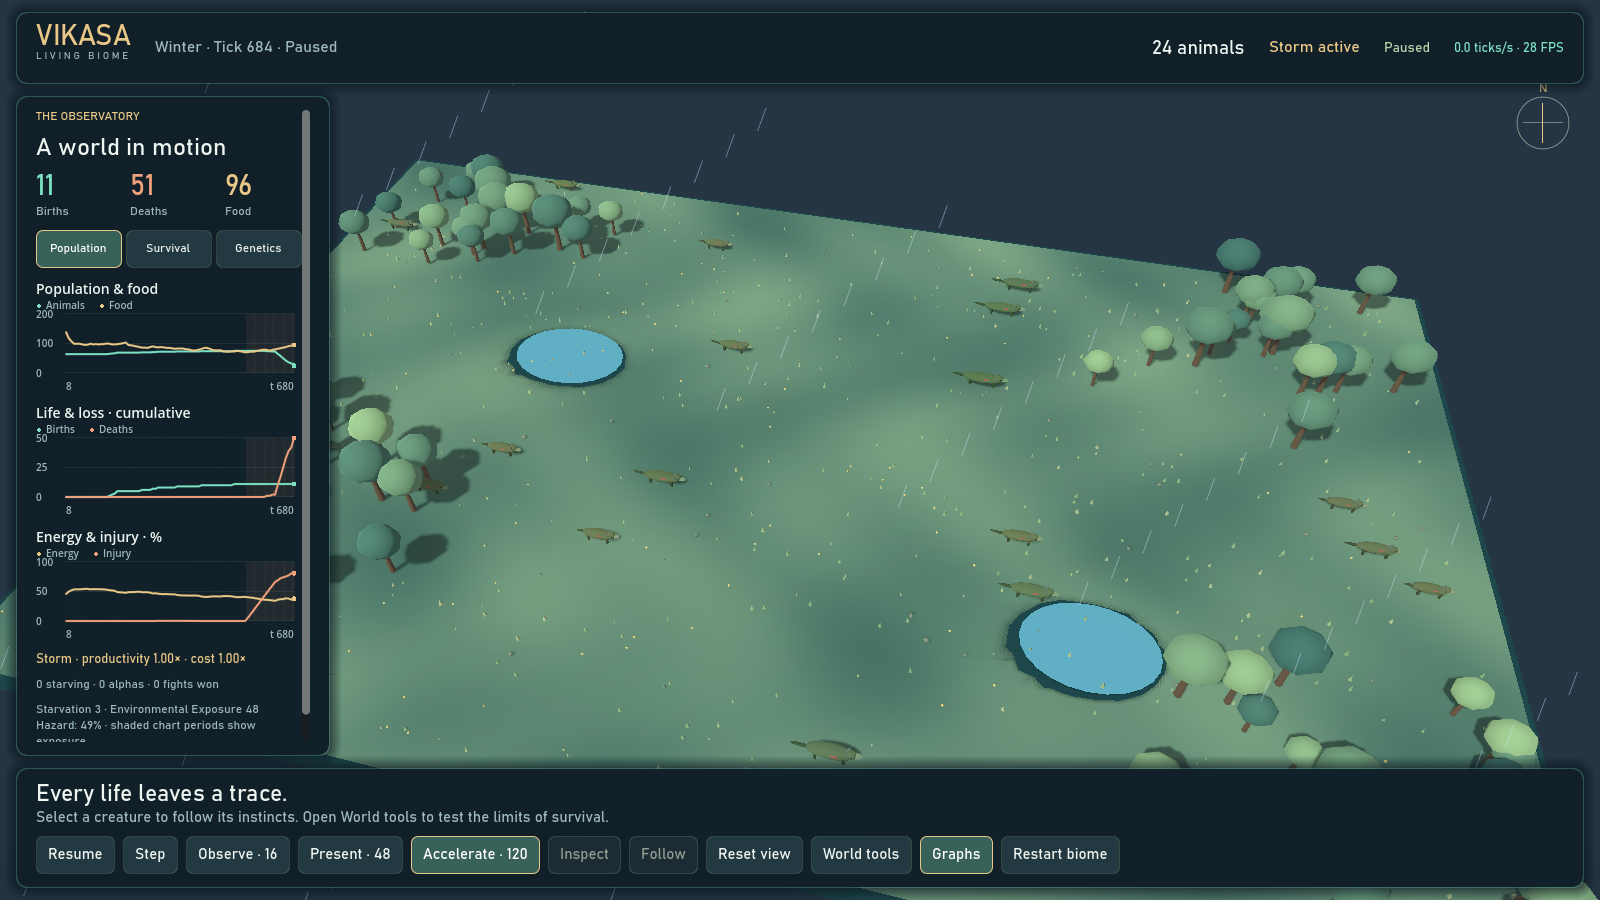
\includegraphics[width=0.6\textwidth]{presentation-storm.png}
\caption{An explicitly applied storm in an older showcase: exposure shading,
falling population and cause-of-death totals.}
\end{figure}

%===========================================================
\chapter{Spatial Plant--Water Ecology}
%===========================================================

The research profile \code{config/spatial-biome.json} replaces abstract food
spawning with a finite $24\times16$ plant-energy field coupled to soil-water
buckets. It is an inspectable conceptual model, not a calibrated hydrological
solver. Each cell carries plant energy $B\in[0,K]$ and dimensionless water
$W\in[0,1]$.

\section{Growth}
Rain first fills available bucket space and evaporation removes only available
water. Local growth is an \emph{exact} logistic step,
\begin{align*}
r_{\text{loc}}&=r\cdot\text{food\_pressure}\cdot\text{seasonal\_productivity}\cdot e^{-((T-0.6)/0.35)^2}\cdot\frac{W}{h+W},\\
B_{\text{growth}}&=\frac{KB}{B+(K-B)e^{-r_{\text{loc}}}}-B,\qquad
\text{water\_used}=\text{transpiration}\cdot B_{\text{growth}}/K,
\end{align*}
limited to what available water can support. Dead cells do not grow and recover
only by transport. Weather removes a fraction $1-e^{-\text{decay}}$ of plant energy.

\section{Transport}
Water and plants undergo a conservative five-point step,
\[
X'=(1-4d)X+d\,(X_N+X_S+X_E+X_W),\qquad 0\le d\le\tfrac14,
\]
a convex combination that preserves non-negativity and maxima. Collision worlds
replicate edges (no flux); wrap worlds use periodic neighbours. Both conserve mass.

\section{Food transfer and audited ledgers}
Natural patch placement picks an eligible cell weighted by plant energy, subtracts
exactly the patch energy and places the patch in that cell; sparse vegetation
yields smaller patches. Cells keep a 1\% seed reservoir, and a 1-unit minimum
transfer bounds negligible fragments. Two identities are audited every run:
\begin{align*}
\text{initial plants}+\text{growth}-\text{weather loss}-\text{harvest}&=\text{current plants},\\
\text{initial water}+\text{infiltrated rain}-\text{evaporation}-\text{transpiration}&=\text{current water}.
\end{align*}
Intentional provisioning is recorded separately as \code{external\_food\_energy}
with an intervention entry (the latest 256 persist). With rainfall 0.004 and no
transpiration or saturation, one 384-tick seasonal cycle adds exactly 0.05952
water per cell; the earlier 0.003 setting lost 0.15936 per cycle.

\begin{figure}[htbp]
\centering
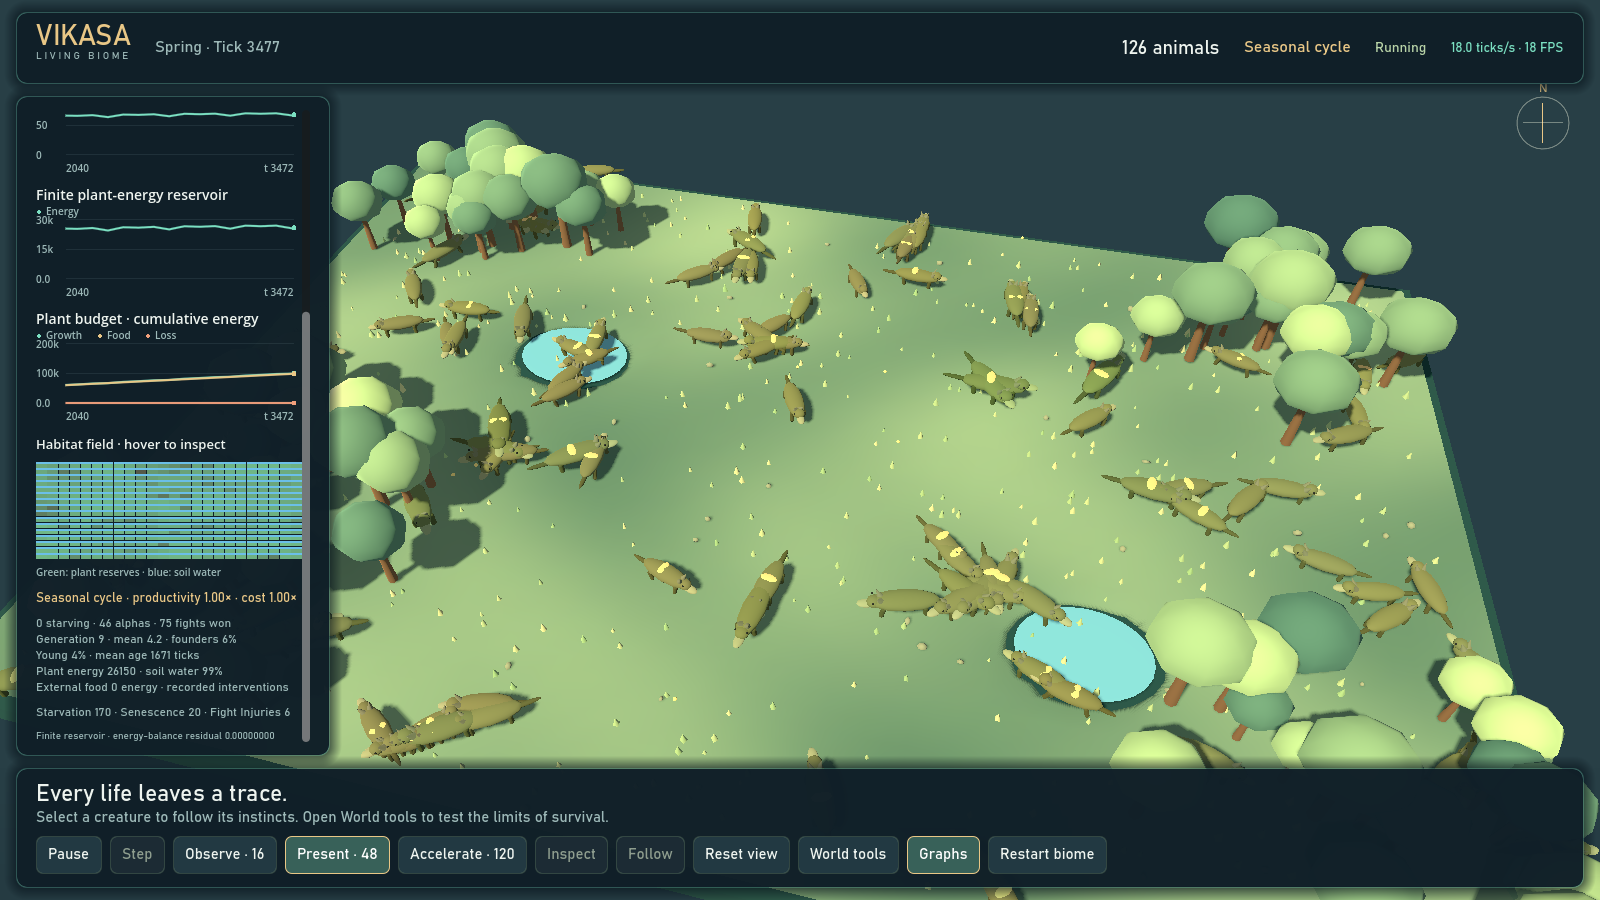
\includegraphics[width=0.9\textwidth]{spatial-ecology.png}
\caption{Ecology tab: plant/water fractions, finite plant reserves, cumulative
growth/harvest/loss, and the interactive cell map (real seed-2026 run).}
\end{figure}

\begin{table}[htbp]
\centering
\caption{Spatial study, 6{,}000 ticks, no rescue or restart}
\begin{tabular}{lcccc}
\toprule
Seed & Living & Births & Deaths & Deepest living generation \\
\midrule
2026 & 131 & 448 & 381 & 16 \\
7 & 130 & 374 & 308 & 11 \\
41 & 129 & 362 & 297 & 12 \\
\bottomrule
\end{tabular}
\end{table}
All three runs survived with no invariant failures; the 95\% Wilson survival
interval is $[0.4385,1.0000]$. Three selected seeds do not establish indefinite
survival or adaptation.
